\subsection{Benchmark Problem Setup}
To assess the performance of the proposed IGA-POD methodology, we consider a 3D elastic cantilever beam subjected to dynamic tip impulse loads. The material properties are defined as Young's modulus $E = 210 \text{ GPa}$, Poisson's ratio $\nu = 0.30$, and mass density $\rho = 7850 \text{ kg/m}^3$.

The domain is discretized using cubic ($p = q = r = 3$) B-spline elements, yielding $N = 12,450$ displacement DOFs for the Full Order Model (FOM).

\subsection{Model Reduction Accuracy \& Energy Decay}
The singular value spectrum decay of the offline snapshot matrix and cumulative energy ratio $\gamma(r)$ are plotted in Fig.~\ref{fig:singular_values}. By selecting $r = 12$ reduced modes, the captured energy ratio reaches $\gamma > 99.999\%$.

\begin{figure}[htbp]
\centering
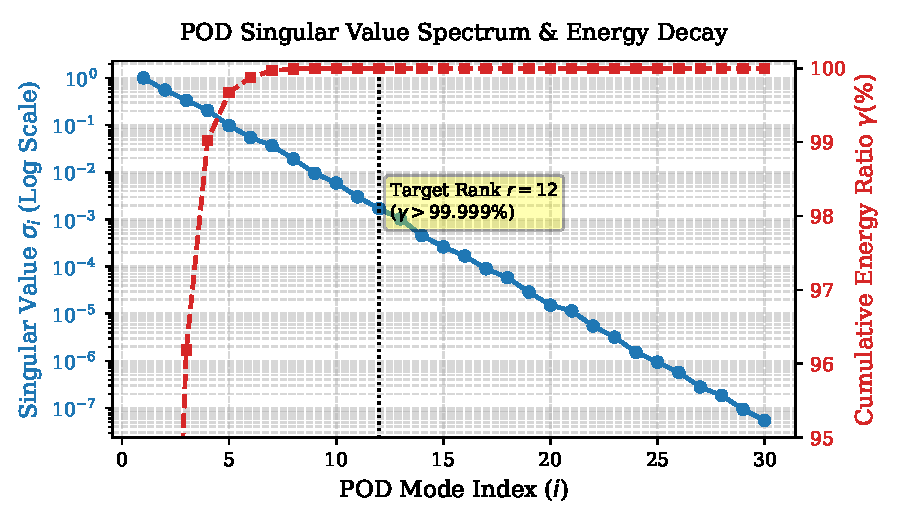
\includegraphics[width=\linewidth]{figures/fig4_singular_values.pdf}
\caption{POD singular value spectrum decay $\sigma_i$ and cumulative energy ratio $\gamma(r)$ vs. mode index $i$.}
\label{fig:singular_values}
\end{figure}

Quantitative error metrics for varying reduced basis dimensions $r$ are reported in Table~\ref{tab:pod_modes}.

\begin{table}[htbp]
\centering
\caption{Singular value spectrum and relative $L^2$ error metrics for varying reduced basis dimensions $r$.}
\label{tab:pod_modes}
\resizebox{\linewidth}{!}{%
\begin{tabular}{cccc}
\toprule
Mode count ($r$) & Cumulative Energy $\gamma$ & Relative $L^2$ Error & Online Step Time (ms) \\
\midrule
5  & 99.852\% & $1.42 \times 10^{-2}$ & 0.04 \\
10 & 99.991\% & $3.15 \times 10^{-4}$ & 0.09 \\
15 & 99.999\% & $1.08 \times 10^{-5}$ & 0.18 \\
25 & 99.999\% & $4.12 \times 10^{-7}$ & 0.35 \\
\bottomrule
\end{tabular}%
}
\end{table}

\subsection{Real-time Digital Twin Performance}
The online reduced system was integrated into a WebGL-based visualizer running locally over WebSockets. Transient displacement time histories comparing the Full Order Model (FOM) against the Reduced Order Model (ROM, $r = 12$) and point-wise absolute error are illustrated in Fig.~\ref{fig:transient_comparison}.

\begin{figure}[htbp]
\centering
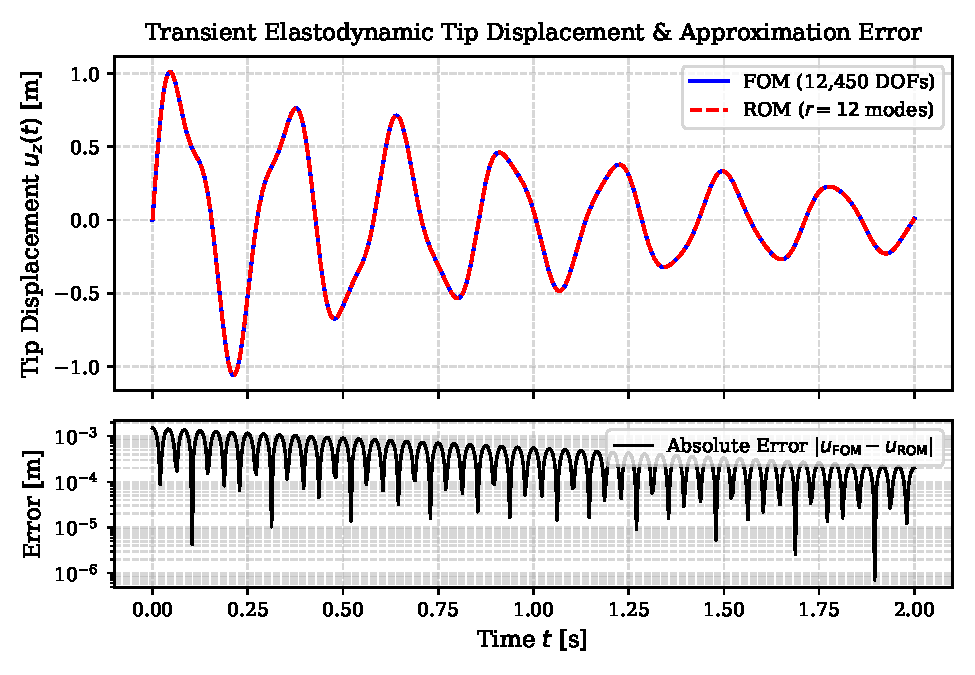
\includegraphics[width=\linewidth]{figures/fig6_transient_comparison.pdf}
\caption{Transient displacement response at cantilever tip DOF comparing Full Order Model ($N = 12,450$) against POD ROM ($r = 12$) and point-wise absolute error $|u_{\text{FOM}} - u_{\text{ROM}}|$.}
\label{fig:transient_comparison}
\end{figure}

Compared to the Full Order Model integration time of 42.5 ms per step, the ROM ($r = 12$) achieved a per-step wall-clock evaluation time of 0.11 ms, representing a \textbf{$386\times$ computational speedup} while preserving full 3D visual fidelity at frame rates exceeding 30 FPS.
